\documentclass[11pt,a4paper]{article}

% Codificacion, idioma y tipografia
\usepackage[utf8]{inputenc}
\usepackage[T1]{fontenc}
\usepackage[spanish, es-nodecimaldot]{babel}
\usepackage{lmodern}

% Pagina y elementos visuales
\usepackage[a4paper, margin=2.5cm]{geometry}
\usepackage{graphicx}
\usepackage{float}
\usepackage{booktabs}
\usepackage{array}
\usepackage{tabularx}
\usepackage{xcolor}
\usepackage{fancyhdr}
\usepackage{caption}
\usepackage{enumitem}
\usepackage{microtype}

% Codigo y enlaces
\usepackage{listings}
\usepackage[hidelinks]{hyperref}

\definecolor{codebg}{RGB}{245,247,250}
\definecolor{codecomment}{RGB}{70,110,70}
\definecolor{codekeyword}{RGB}{35,75,150}

\lstdefinelanguage{CQL}{
	morekeywords={SELECT,FROM,WHERE,AND,LIMIT,ORDER,BY,ASC,DESC,CREATE,KEYSPACE,
		TABLE,INDEX,ON,USING,WITH,PRIMARY,KEY,CLUSTERING,INSERT,INTO,VALUES,
		USE,TRACING,ALLOW,FILTERING,CONTAINS,STATIC,DESCRIBE,UPDATE,SET,DROP,
		CONSISTENCY,text,int,uuid,date,bigint,set},
	sensitive=false,
	morecomment=[l]{--},
	morestring=[b]'
}

\lstset{
	language=CQL,
	inputencoding=utf8,
	extendedchars=true,
	basicstyle=\ttfamily\small,
	keywordstyle=\color{codekeyword}\bfseries,
	commentstyle=\color{codecomment},
	backgroundcolor=\color{codebg},
	frame=single,
	rulecolor=\color{black!20},
	breaklines=true,
	keepspaces=true,
	columns=fullflexible,
	showstringspaces=false,
	numbers=left,
	numberstyle=\tiny\color{black!50},
	xleftmargin=1.5em,
	framexleftmargin=1.2em,
	literate={á}{{\'a}}1 {é}{{\'e}}1 {í}{{\'i}}1 {ó}{{\'o}}1 {ú}{{\'u}}1
	          {Á}{{\'A}}1 {É}{{\'E}}1 {Í}{{\'I}}1 {Ó}{{\'O}}1 {Ú}{{\'U}}1
	          {ñ}{{\~n}}1 {Ñ}{{\~N}}1 {ü}{{\"u}}1 {Ü}{{\"U}}1
	          {¿}{{?`}}1 {¡}{{!`}}1
}

\setlist{nosep}
\setlength{\parindent}{0pt}
\setlength{\parskip}{0.6em}

\pagestyle{fancy}
\fancyhf{}
\lhead{Bases de Datos Avanzadas}
\rhead{Tarea 2: Apache Cassandra}
\cfoot{\thepage}

\begin{document}

\begin{titlepage}
	\centering
	\vspace*{1cm}
	{\Large Universidad Técnica Federico Santa María\\}
	{\large Campus Santiago San Joaquín\\[0.3em]
	Bases de Datos Avanzadas\\[3cm]}
	{\Huge\bfseries Tarea 2: Apache Cassandra\\[1.5cm]}
	{\Large Informe\par}
	\vfill
	\begin{tabular}{rl}
		\textbf{Nombre:} & Sebastián Andrés Santander Martínez\\
		\textbf{Rol:} & 202373608-2\\[0.5em]
		\textbf{Nombre:} & Jaime Guzmán\\
		\textbf{Rol:} & (pendiente)\\
	\end{tabular}
	\vfill
	Segundo semestre 2026
\end{titlepage}

\tableofcontents
\newpage

\section{Introducción}

En este informe se repite el caso de Voice Managers de la tarea anterior, pero ahora sobre
Apache Cassandra. La diferencia principal con MongoDB es que en Cassandra las tablas se
diseñan a partir de las consultas que va a hacer la aplicación.

Se trabajó con un clúster de tres nodos levantado con Docker, un keyspace con factor de
replicación 3 y tres tablas pensadas para las consultas pedidas. Sobre eso se analizaron las
consultas con \texttt{TRACING}, se probó \texttt{ALLOW FILTERING}, se crearon índices SAI y
se comparó la desnormalización con el uso de índices.

Los archivos de la tarea (\texttt{schema.cql}, el script de generación de datos, las
consultas y las capturas) están en el repositorio público
\url{https://github.com/Sxbayb/Tareas-BDDA}.

\section{Preparación del entorno}

\subsection{Clúster de Cassandra}

El clúster se levantó con el \texttt{docker-compose.yml} entregado en Aula, que define tres
contenedores con Cassandra 5.0 (\texttt{cassandra1}, \texttt{cassandra2} y \texttt{cassandra3}).

\begin{lstlisting}[language={}]
docker compose up -d
docker exec -it cassandra1 nodetool status
\end{lstlisting}

En el primer intento los tres contenedores se detuvieron a los pocos segundos con código de
salida 137, que corresponde a un proceso terminado por falta de memoria. El log mostraba que
Cassandra partía con 512 MB de heap y 256 MB de memoria directa, pero a eso se suma la memoria
que usa la JVM, código compilado y más, con lo que el límite de 1 GB por contenedor no alcanzaba. Se subió
\texttt{mem\_limit} a \texttt{1536m} en los tres nodos, sin tocar el heap, y se levantaron
de a uno esperando que cada nodo quedara en estado \texttt{UN} antes de iniciar el siguiente.

\begin{figure}[H]
	\centering
	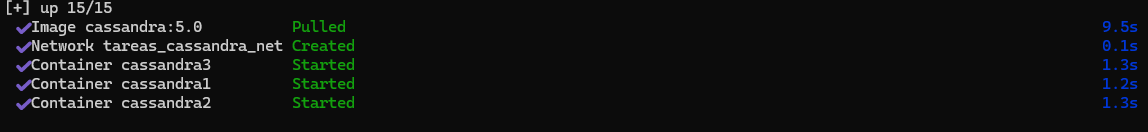
\includegraphics[width=0.7\textwidth]{img/nodosIniciales.png}
	\caption{Creación de la red y de los tres contenedores con Docker Compose.}
	\label{fig:compose}
\end{figure}

\begin{figure}[H]
	\centering
	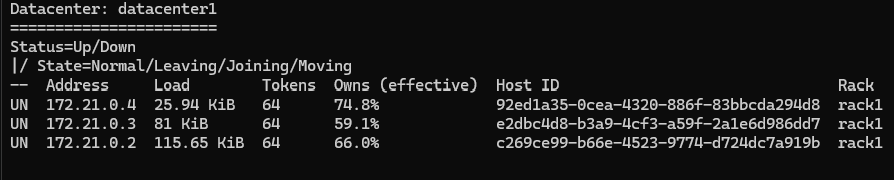
\includegraphics[width=0.85\textwidth]{img/setup_nodetool.png}
	\caption{Los tres nodos del clúster en estado UN (Up/Normal).}
	\label{fig:nodetool}
\end{figure}

\subsection{Keyspace}

Antes de crear el keyspace se consultó el nombre del datacenter, que resultó ser
\texttt{datacenter1}.

\begin{figure}[H]
	\centering
	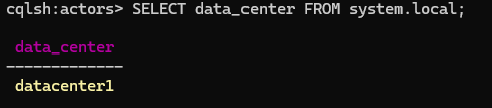
\includegraphics[width=0.45\textwidth]{img/datacenter.png}
	\caption{Nombre del datacenter obtenido desde \texttt{system.local}.}
	\label{fig:datacenter}
\end{figure}

El keyspace \texttt{actors} se creó con \texttt{NetworkTopologyStrategy} y factor de
replicación 3. Como el clúster tiene tres nodos, cada nodo guarda una copia completa de los
datos.

\begin{lstlisting}
CREATE KEYSPACE IF NOT EXISTS actors
WITH replication = {
    'class': 'NetworkTopologyStrategy',
    'datacenter1': 3
};
\end{lstlisting}

\begin{figure}[H]
	\centering
	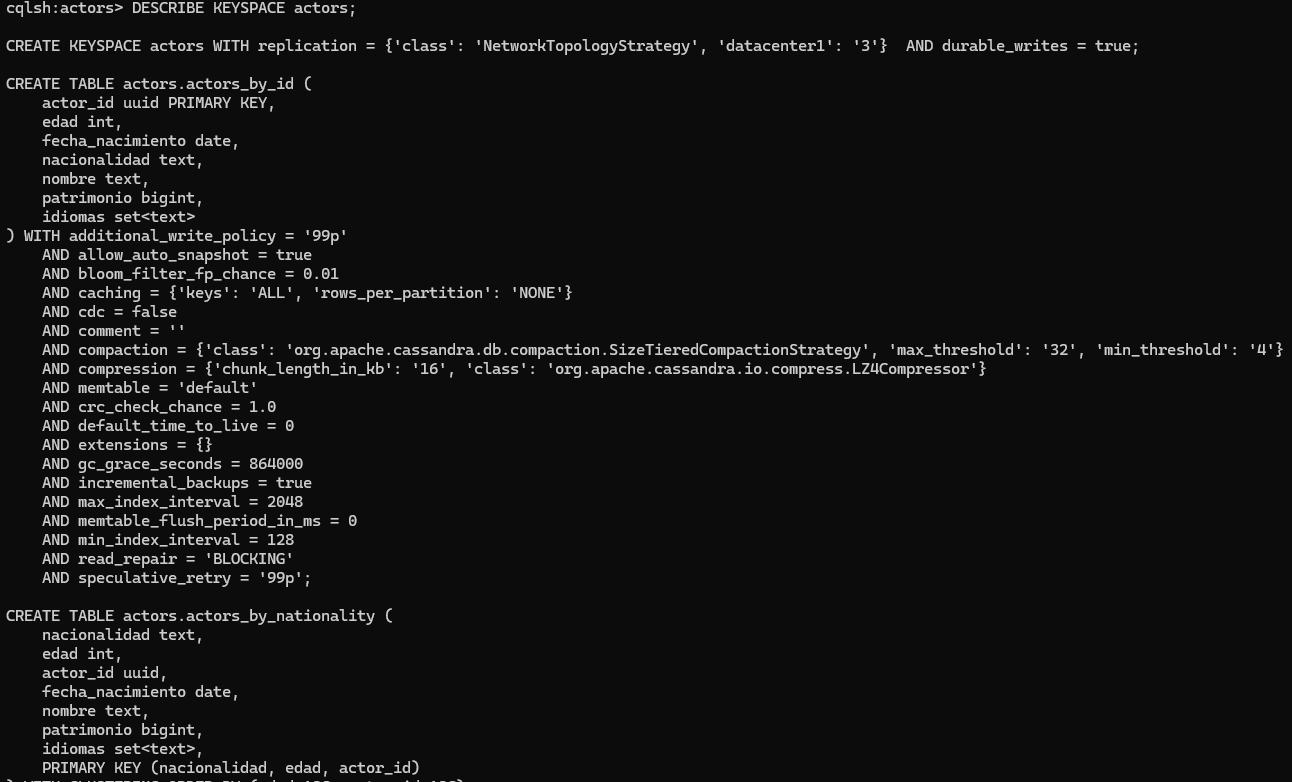
\includegraphics[width=\textwidth]{img/setup_keyspace.png}
	\caption{Resultado de \texttt{DESCRIBE KEYSPACE actors} con la estrategia de replicación.}
	\label{fig:keyspace}
\end{figure}

\section{Preparación de los datos y diseño de las tablas}

\subsection{Diseño orientado a consultas}

Las tablas se diseñaron a partir de las tres consultas mínimas del enunciado. Cada tabla
resuelve una consulta usando solo su clave primaria.

\begin{table}[H]
	\centering
	\small
	\begin{tabularx}{\textwidth}{>{\ttfamily}l X X X}
		\toprule
		\textnormal{\textbf{Tabla}} & \textbf{PRIMARY KEY} & \textbf{Partición / clustering} & \textbf{Consulta que resuelve} \\
		\midrule
		actors\_by\_id & \texttt{(actor\_id)} & Partición: \texttt{actor\_id}. Sin clustering. & Obtener un actor por su identificador. \\
		\addlinespace
		actors\_by\_nationality & \texttt{((nacionalidad), edad, actor\_id)} & Partición: \texttt{nacionalidad}. Clustering: \texttt{edad} ASC y \texttt{actor\_id}. & Actores de una nacionalidad ordenados por edad. \\
		\addlinespace
		characters\_by\_actor & \texttt{((actor\_id), rol, apariciones, nombre\_personaje)} & Partición: \texttt{actor\_id}. Clustering: \texttt{rol}, \texttt{apariciones} DESC y \texttt{nombre\_personaje}. & Personajes de un actor filtrando por rol y ordenados por apariciones. \\
		\bottomrule
	\end{tabularx}
	\caption{Tablas del keyspace \texttt{actors}.}
	\label{tab:diseno}
\end{table}

En \texttt{actors\_by\_nationality} se agregó \texttt{actor\_id} al final del clustering
porque dos actores del mismo país pueden tener la misma edad. Sin esa columna la clave sería
la misma y el segundo \texttt{INSERT} sobrescribiría al primero, ya que en Cassandra un
\texttt{INSERT} con una clave existente funciona como una actualización. Por la misma razón
\texttt{nombre\_personaje} cierra la clave de \texttt{characters\_by\_actor}.

En \texttt{characters\_by\_actor} el orden de las columnas de clustering importa. \texttt{rol}
va primero para poder filtrar por igualdad (\texttt{rol = 'Principal'}) y \texttt{apariciones}
va después con orden descendente, así que dentro de cada rol los personajes quedan guardados
de mayor a menor. La columna \texttt{nombre\_actor} se declaró \texttt{STATIC}, por lo que se
guarda una sola vez por partición y no se repite en cada personaje.

Hay información duplicada. Nombre, fecha de nacimiento, patrimonio e idiomas están tanto en
\texttt{actors\_by\_id} como en \texttt{actors\_by\_nationality}. Esa duplicación es la que
permite responder la consulta por nacionalidad leyendo una sola partición, a cambio de tener
que actualizar ambas tablas cuando cambia alguno de esos datos.

Las tres tablas están en \texttt{schema.cql}. Como ejemplo, la tabla de personajes:

\begin{lstlisting}
CREATE TABLE IF NOT EXISTS characters_by_actor (
    actor_id          uuid,
    rol               text,
    apariciones       int,
    nombre_personaje  text,
    nombre_actor      text STATIC,
    produccion        text,
    tipo_produccion   text,
    generos           set<text>,
    PRIMARY KEY ((actor_id), rol, apariciones, nombre_personaje)
) WITH CLUSTERING ORDER BY (rol ASC, apariciones DESC, nombre_personaje ASC);
\end{lstlisting}

\subsection{Generación y carga de datos}

Los datos se generaron con \texttt{generar\_datos.py}, que usa la biblioteca Faker con una
semilla fija. El script crea 24 actores ficticios con identificador, nombre, nacionalidad,
fecha de nacimiento, edad, patrimonio, idiomas (\texttt{set<text>}) y entre uno y siete
personajes, cada uno con nombre, producción, tipo, rol, apariciones y géneros.

Algunos valores se fijaron a propósito para que las consultas tuvieran resultados útiles.

El identificador es un UUID y en Cassandra no hay autoincremento,
porque en un sistema distribuido ningún nodo lleva la cuenta global de los ids.

El script escribe directamente \texttt{datos.cql} con los \texttt{INSERT} de las tres tablas.
Cada actor se inserta dos veces (en \texttt{actors\_by\_id} y en
\texttt{actors\_by\_nationality}) y cada personaje es una fila de
\texttt{characters\_by\_actor}, en total 112 \texttt{INSERT}. Los archivos se copiaron al
contenedor y se ejecutaron con \texttt{cqlsh -f}.

\begin{lstlisting}[language={}]
docker cp schema.cql cassandra1:/tmp/schema.cql
docker exec -it cassandra1 cqlsh -f /tmp/schema.cql
docker cp datos.cql cassandra1:/tmp/datos.cql
docker exec -it cassandra1 cqlsh -f /tmp/datos.cql
\end{lstlisting}

\begin{figure}[H]
	\centering
	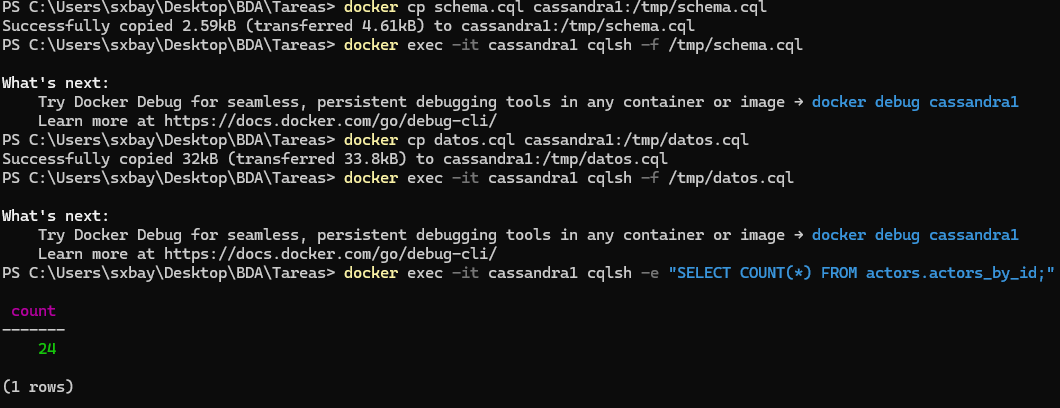
\includegraphics[width=0.85\textwidth]{img/datos_count.png}
	\caption{Carga del esquema y de los datos, y conteo de los 24 actores.}
	\label{fig:carga}
\end{figure}

El \texttt{COUNT(*)} sin clave de partición genera advertencia, porque para contar tiene que recorrer
todas las particiones. Con 24 filas no importa, pero es el mismo problema que aparece más
adelante con \texttt{ALLOW FILTERING}.

\begin{figure}[H]
	\centering
	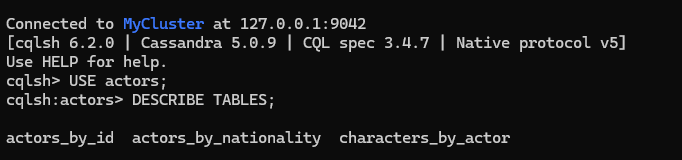
\includegraphics[width=0.65\textwidth]{img/ingreso_cqlsh.png}
	\caption{Ingreso a \texttt{cqlsh} y tablas creadas en el keyspace.}
	\label{fig:cqlsh}
\end{figure}

\section{Parte 1: Consultas}

En todas las consultas se usó como ejemplo a la actriz Josefa Brenda Alarcón Álvarez, con
\texttt{actor\_id} \texttt{8c53765f-4ec0-4954-bf8b-2a6aab74fe57}.

\subsection{Búsqueda por clave de partición}

\begin{lstlisting}
SELECT nombre, nacionalidad, edad, idiomas
FROM actors_by_id
WHERE actor_id = 8c53765f-4ec0-4954-bf8b-2a6aab74fe57;
\end{lstlisting}

\begin{figure}[H]
	\centering
	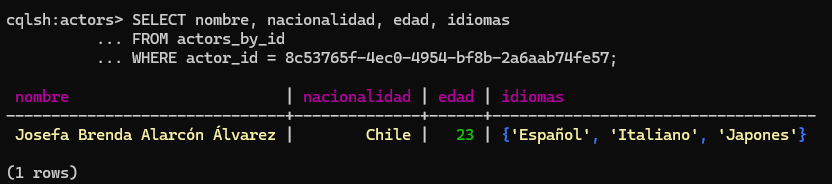
\includegraphics[width=0.75\textwidth]{img/P1_consulta1.png}
	\caption{Actor obtenido por su identificador.}
	\label{fig:p1c1}
\end{figure}

\textbf{Explicación:} \texttt{actor\_id} es la clave de partición de la tabla. Cassandra
aplica la función hash sobre el id, obtiene un token y con eso sabe exactamente qué
nodos tienen esa partición. No necesita revisar ninguna otra partición, así que el costo de la
consulta no depende de cuántos actores haya en la tabla. Los idiomas aparecen en orden
alfabético porque un \texttt{set} se guarda ordenado.

\subsection{Consulta por nacionalidad}

\begin{lstlisting}
SELECT nombre, edad, nacionalidad
FROM actors_by_nationality
WHERE nacionalidad = 'Chile'
LIMIT 10;
\end{lstlisting}

\begin{figure}[H]
	\centering
	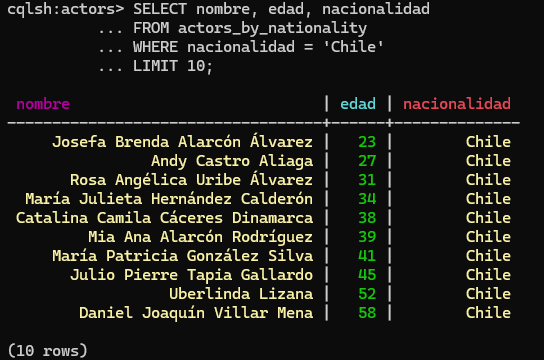
\includegraphics[width=0.55\textwidth]{img/P1_consulta2.png}
	\caption{Actores chilenos ordenados por edad.}
	\label{fig:p1c2}
\end{figure}

\textbf{Explicación:} \texttt{nacionalidad} es la clave de partición, por lo que todos los
actores chilenos están juntos en la misma partición. \texttt{edad} es la primera columna de
clustering, y las filas ya están guardadas en disco ordenadas por edad. Por eso el resultado
sale ordenado sin escribir \texttt{ORDER BY}. El \texttt{LIMIT 10} deja fuera a dos
chilenos.

\subsection{Consulta de personajes}

\begin{lstlisting}
SELECT nombre_actor, nombre_personaje, rol, apariciones, produccion
FROM characters_by_actor
WHERE actor_id = 8c53765f-4ec0-4954-bf8b-2a6aab74fe57
  AND rol = 'Principal'
LIMIT 10;
\end{lstlisting}

\begin{figure}[H]
	\centering
	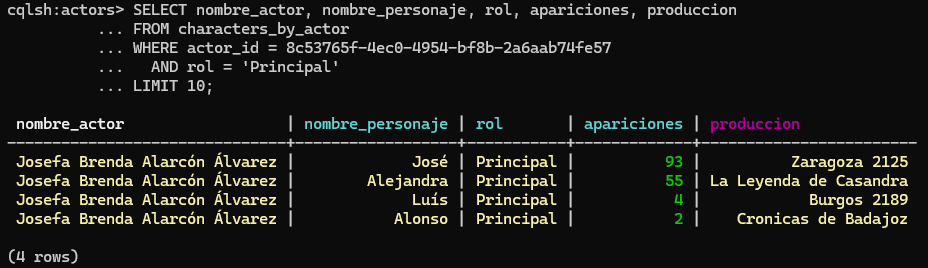
\includegraphics[width=0.9\textwidth]{img/P1_consulta3.png}
	\caption{Personajes principales ordenados por apariciones.}
	\label{fig:p1c3}
\end{figure}

\textbf{Explicación:} la consulta entrega la partición completa (\texttt{actor\_id}) y una
igualdad sobre la primera columna de clustering (\texttt{rol}). Dentro de la partición, las
filas con rol Principal forman un bloque contiguo, ya ordenado por \texttt{apariciones} de
mayor a menor (93, 55, 4 y 2) gracias al \texttt{CLUSTERING ORDER BY} definido al crear la
tabla. La consulta se resuelve solo con la clave primaria.

\subsection{LIMIT y ordenamiento}

\begin{lstlisting}
SELECT nombre, edad
FROM actors_by_nationality
WHERE nacionalidad = 'Chile'
ORDER BY edad DESC
LIMIT 5;
\end{lstlisting}

\begin{figure}[H]
	\centering
	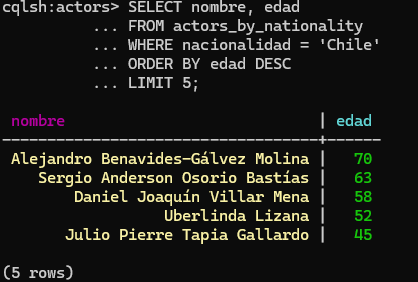
\includegraphics[width=0.45\textwidth]{img/P1_consulta4.png}
	\caption{Los cinco actores chilenos de mayor edad.}
	\label{fig:p1c4}
\end{figure}

Para comprobar que no se puede ordenar por cualquier columna se intentó ordenar por patrimonio:

\begin{lstlisting}
SELECT nombre, patrimonio
FROM actors_by_nationality
WHERE nacionalidad = 'Chile'
ORDER BY patrimonio DESC
LIMIT 5;
\end{lstlisting}

\begin{figure}[H]
	\centering
	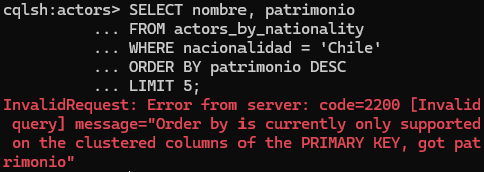
\includegraphics[width=0.5\textwidth]{img/P1_consulta_error.png}
	\caption{Error al ordenar por una columna que no es de clustering.}
	\label{fig:p1c4error}
\end{figure}

\textbf{Explicación:} Dentro de una partición Cassandra puede leer las filas en el orden del
clustering o en el orden inverso. \texttt{ORDER BY edad DESC} solo invierte la lectura, así
que Cassandra recorre la partición desde el final y se detiene en la quinta fila.
\texttt{patrimonio} no es columna de clustering, y para ordenar por ella Cassandra tendría que
leer toda la partición y ordenarla en memoria. Por eso responde \textit{Order by is currently
only supported on the clustered columns of the PRIMARY KEY}.

En una base de datos relacional se puede ordenar por cualquier columna porque trabaja
sobre un solo servidor y aplica un sort al resultado. Cassandra evita ese trabajo a propósito,
porque en una tabla distribuida con millones de filas un ordenamiento en memoria sería caro e
impredecible. El orden se decide al diseñar la tabla, y si se necesita otro orden se crea otra
tabla con un clustering distinto.

\section{Parte 2: Procesamiento de consultas y diseño}

Para leer los resultados de esta parte hay que saber qué dirección corresponde a cada nodo.
cqlsh estaba conectado a \texttt{cassandra1}, por lo que ese nodo actuó como coordinador en
todas las consultas.

\begin{table}[H]
	\centering
	\begin{tabular}{ll}
		\toprule
		\textbf{Dirección} & \textbf{Nodo} \\
		\midrule
		172.21.0.2 & cassandra1 (coordinador) \\
		172.21.0.3 & cassandra2 \\
		172.21.0.4 & cassandra3 \\
		\bottomrule
	\end{tabular}
	\caption{Direcciones de los nodos del clúster.}
	\label{tab:ips}
\end{table}

\subsection{TRACING}

Se activó \texttt{TRACING ON} y se repitieron las tres primeras consultas de la Parte 1.

\begin{figure}[H]
	\centering
	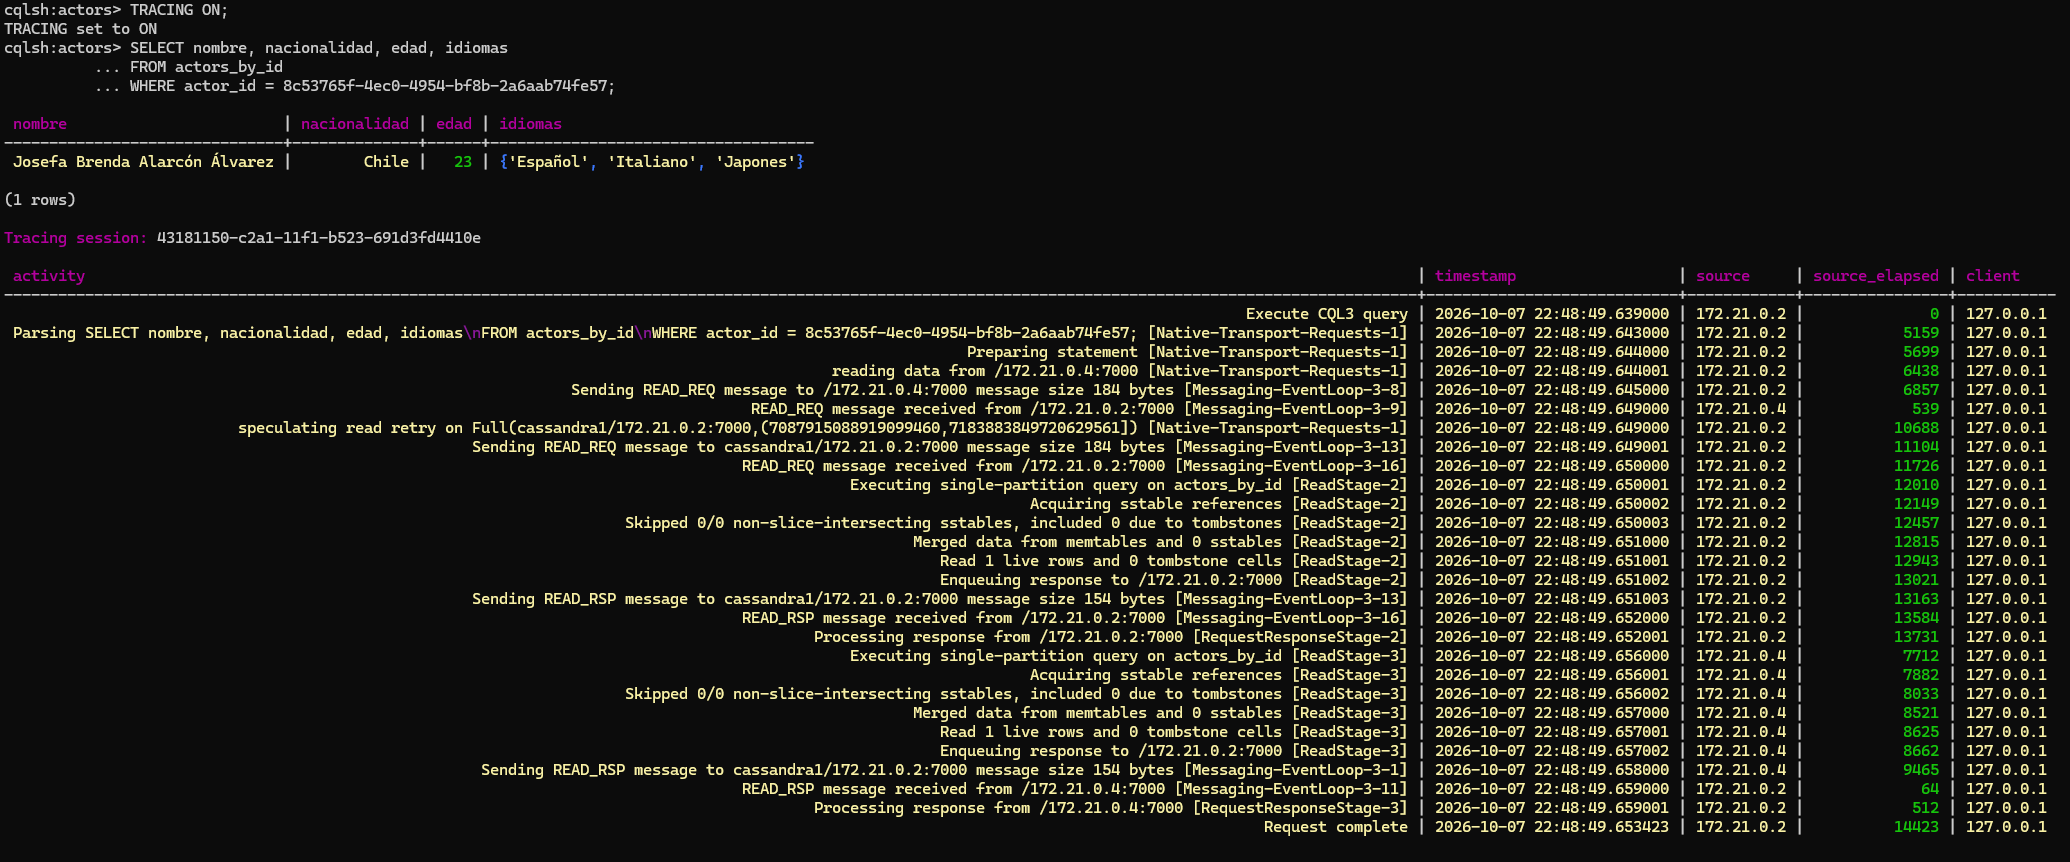
\includegraphics[width=\textwidth]{img/P2_tracing1.png}
	\caption{Tracing de la búsqueda por \texttt{actor\_id}.}
	\label{fig:tracing1}
\end{figure}

\begin{figure}[H]
	\centering
	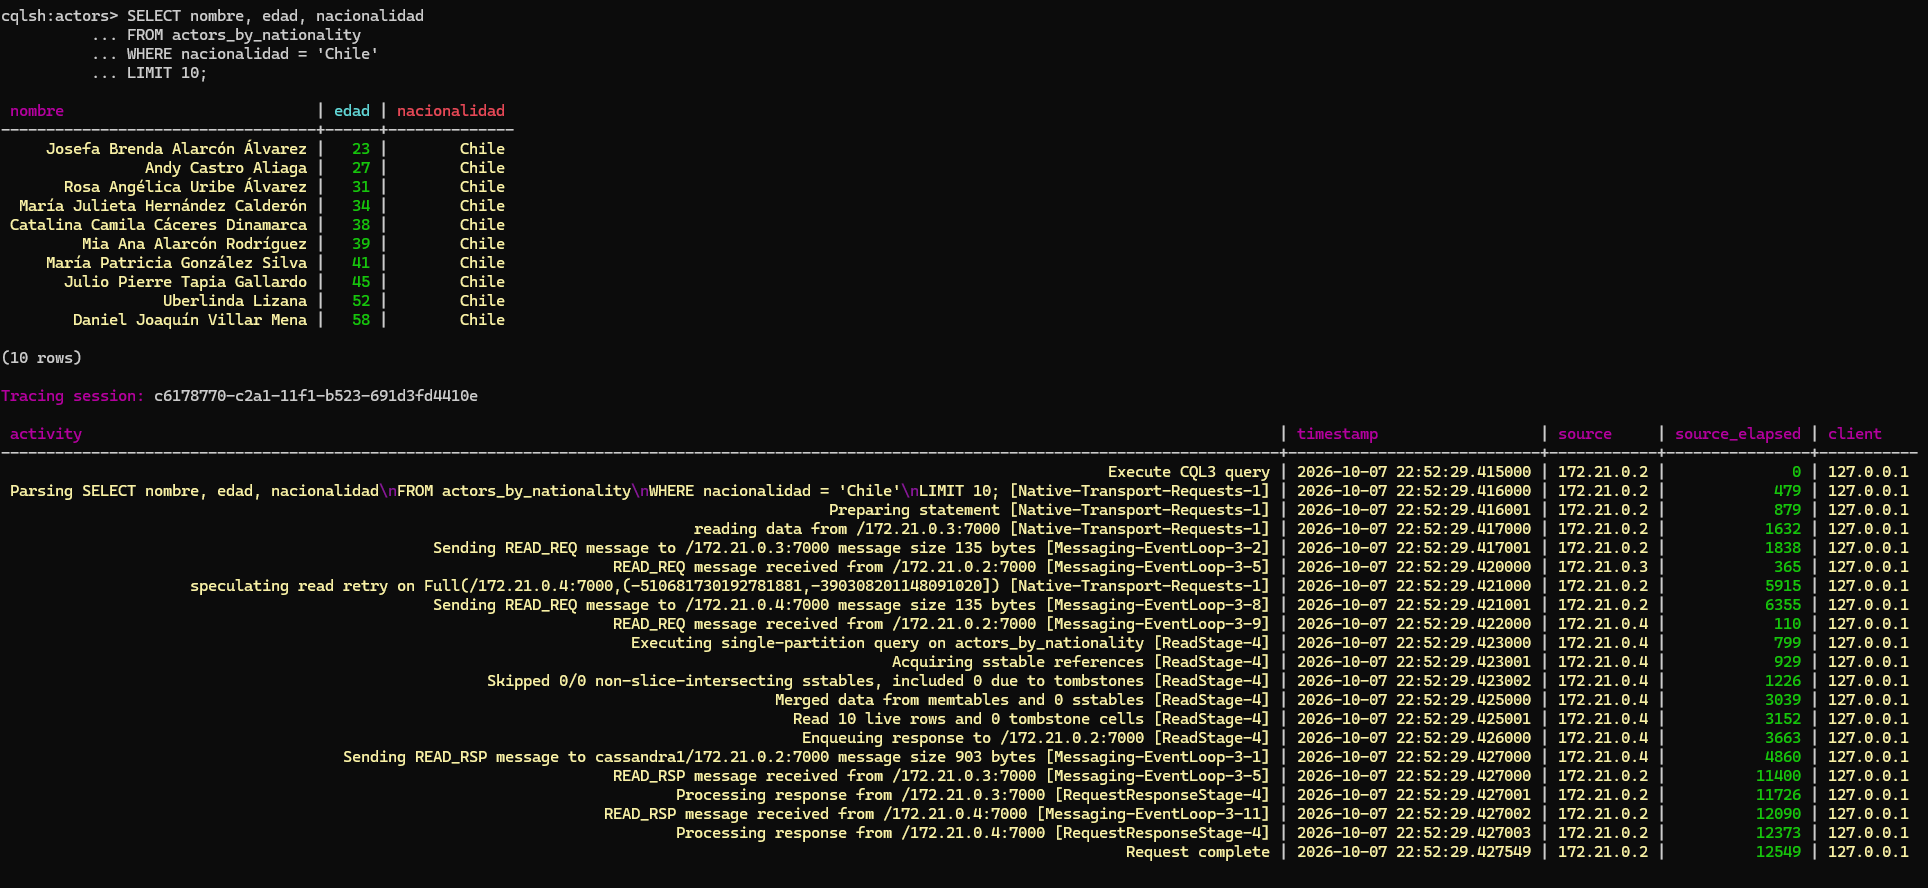
\includegraphics[width=\textwidth]{img/P2_tracing2.png}
	\caption{Tracing de la consulta por nacionalidad en \texttt{actors\_by\_nationality}.}
	\label{fig:tracing2}
\end{figure}

\begin{figure}[H]
	\centering
	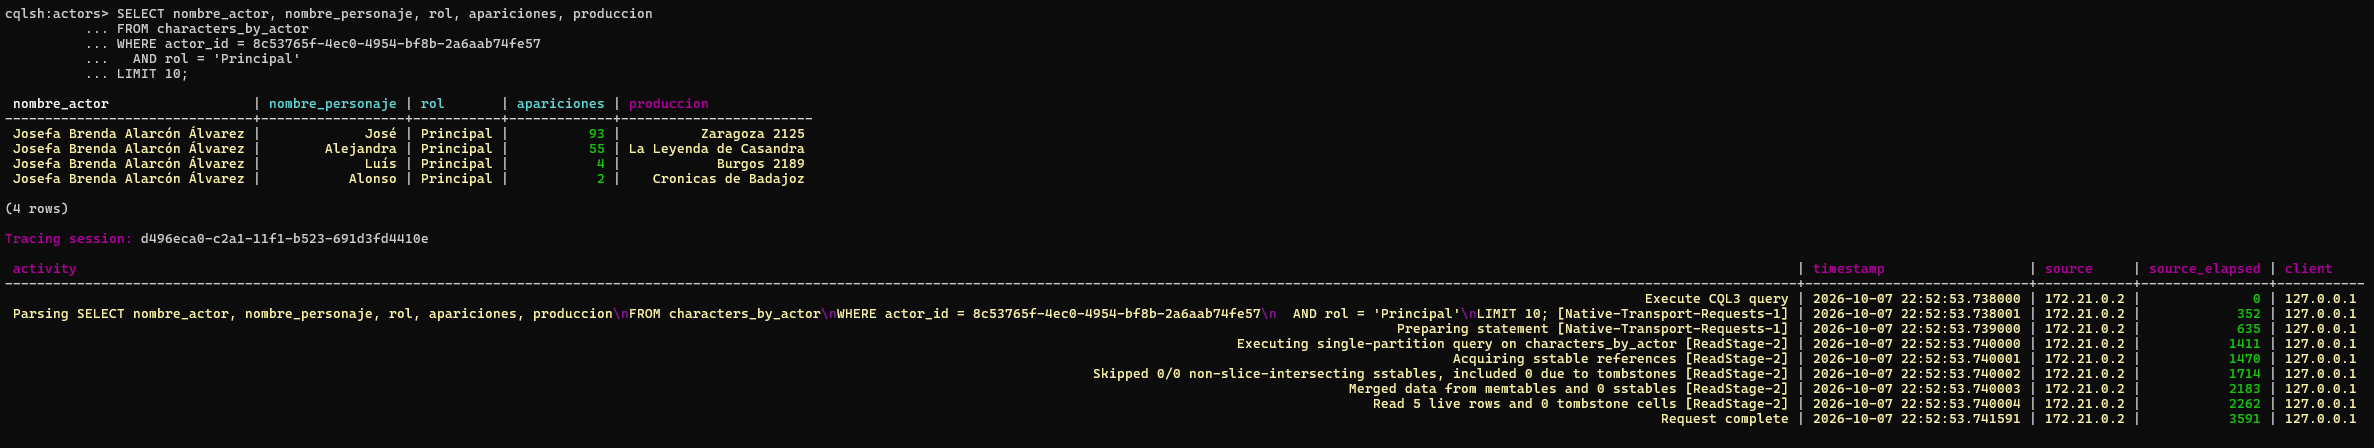
\includegraphics[width=\textwidth]{img/P2_tracing3.png}
	\caption{Tracing de la consulta de personajes principales.}
	\label{fig:tracing3}
\end{figure}

\begin{table}[H]
	\centering
	\small
	\begin{tabularx}{\textwidth}{l l X l r}
		\toprule
		\textbf{Consulta} & \textbf{Coordinador} & \textbf{Nodos que leyeron} & \textbf{Filas leídas} & \textbf{Tiempo} \\
		\midrule
		1.1 por \texttt{actor\_id} & cassandra1 & cassandra3 y cassandra1 (lectura especulativa) & 1 & 14,4 ms \\
		1.2 por nacionalidad & cassandra1 & cassandra2 y cassandra3 (lectura especulativa) & 10 & 12,5 ms \\
		1.3 personajes & cassandra1 & solo cassandra1 (lectura local) & 5 & 3,6 ms \\
		\bottomrule
	\end{tabularx}
	\caption{Resumen de los tracings de la Parte 1.}
	\label{tab:tracing}
\end{table}

\textbf{Nodo coordinador y nodos involucrados.} En las tres consultas el coordinador fue
cassandra1, el nodo al que estaba conectado cqlsh. El coordinador recibe la consulta, la
parsea, calcula el token de la clave departición y decide a qué réplica pedirle los datos. 
Como el keyspace tiene RF = 3 con tres
nodos, cualquier nodo es réplica de cualquier partición.

En la consulta 1.1 el coordinador envió un \texttt{READ\_REQ} a cassandra3. Poco después
aparece \textit{speculating read retry}: al no recibir respuesta dentro del tiempo esperado,
el coordinador mandó la misma lectura a otra réplica, en este caso a sí mismo. Esto viene de
la propiedad \texttt{speculative\_retry = '99p'} de la tabla, visible en la
Figura~\ref{fig:keyspace}, y sirve para no quedar esperando a una réplica lenta. En la 1.2
pasó lo mismo con cassandra2 y cassandra3. En la 1.3 no hubo mensajes entre nodos, porque el
coordinador leyó su propia copia.

\textbf{Operaciones realizadas.} Las tres consultas muestran \textit{Executing single-partition
query}, es decir, cada una leyó una sola partición. La línea \textit{Read N live rows} indica
cuántas filas se leyeron: 1 en la búsqueda por id, 10 en la consulta por nacionalidad (las
primeras diez del orden del clustering) y 5 en la de personajes (los cuatro personajes
principales más, probablemente, la fila estática con \texttt{nombre\_actor}). 

Las tres consultas terminaron entre 3,6 y 14,4 ms. La 1.3 fue la
más rápida porque se resolvió de forma local, sin red. En las otras dos la mayor parte del
tiempo se fue en el envío de mensajes entre nodos y en la lectura especulativa.

Las tres consultas entregan la
clave de partición completa, por eso Cassandra sabe de antemano qué partición leer y no
consulta rangos del anillo. El clustering se nota en que ninguna necesitó ordenar: la 1.2 leyó
las diez primeras filas de la partición de Chile, que ya estaban ordenadas por edad, y la 1.3
leyó un bloque contiguo dentro de la partición del actor.

\subsection{Consulta sin clave apropiada}

Sobre la tabla principal se intentó filtrar por nacionalidad y edad, columnas que no forman
parte de su clave primaria.

\begin{lstlisting}
SELECT nombre, nacionalidad, edad
FROM actors_by_id
WHERE nacionalidad = 'Chile' AND edad > 40
LIMIT 10;
\end{lstlisting}

\begin{figure}[H]
	\centering
	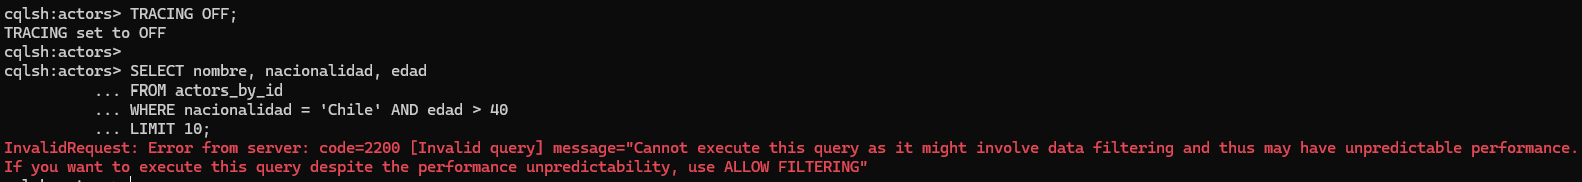
\includegraphics[width=\textwidth]{img/P2_sin_clave_error.png}
	\caption{Cassandra rechaza la consulta sin clave de partición.}
	\label{fig:sinclave}
\end{figure}

Cassandra respondió \textit{Cannot execute this query as it might involve data filtering and
thus may have unpredictable performance}. Luego se repitió la consulta agregando
\texttt{ALLOW FILTERING} y con \texttt{TRACING ON}.

\begin{lstlisting}
SELECT nombre, nacionalidad, edad
FROM actors_by_id
WHERE nacionalidad = 'Chile' AND edad > 40
LIMIT 10
ALLOW FILTERING;
\end{lstlisting}

\begin{figure}[H]
	\centering
	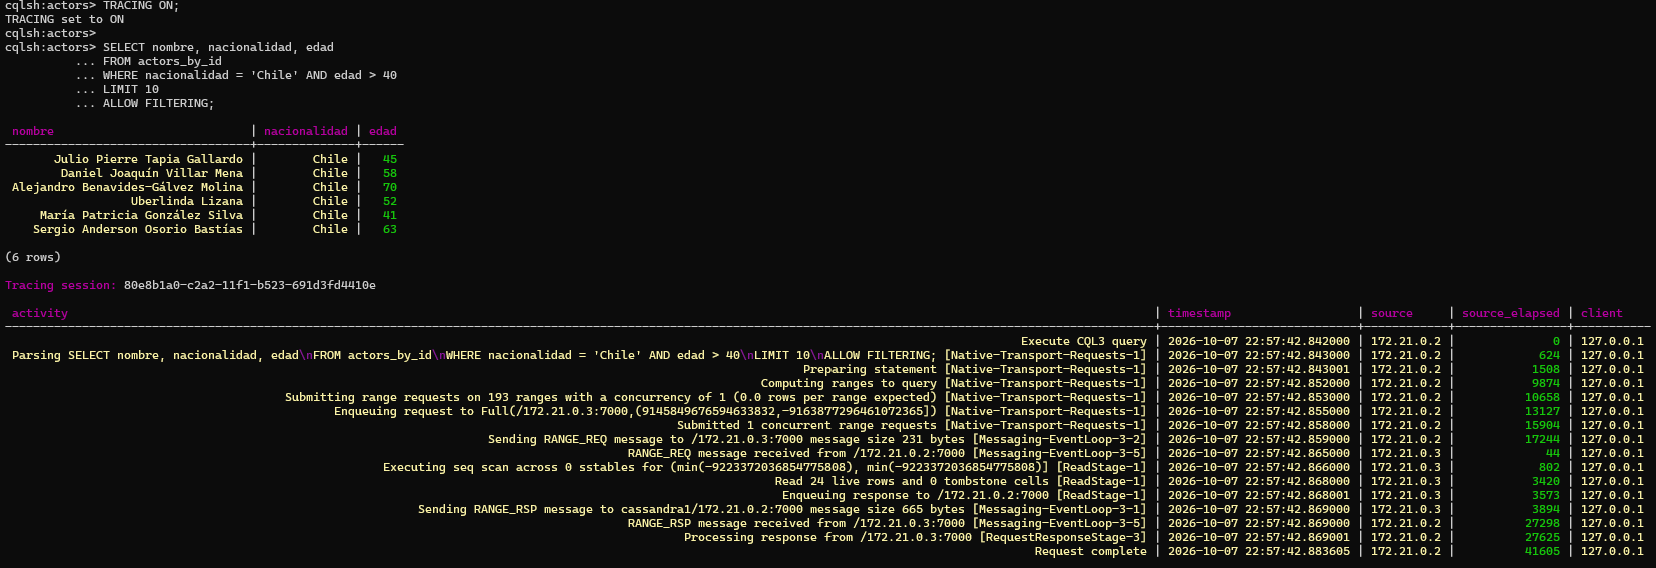
\includegraphics[width=\textwidth]{img/P2_allow_filtering.png}
	\caption{Resultado y tracing con \texttt{ALLOW FILTERING}.}
	\label{fig:allowfiltering}
\end{figure}

El tracing es muy distinto a los anteriores. Ya no aparece \textit{single-partition query}
sino \textit{Submitting range requests on 193 ranges}, es decir, el coordinador tuvo que
consultar todos los rangos de tokens del anillo. Luego aparece \textit{Executing seq scan}
sobre el rango que va desde el token mínimo hasta el mínimo, o sea la tabla completa, y
\textit{Read 24 live rows}. Cassandra leyó los 24 actores para devolver solo 6, y las otras 18
filas se leyeron y se descartaron. La consulta tardó 41,6 ms, entre tres y once veces más que
las consultas por clave. Además el resultado sale desordenado,
porque en esta tabla el orden lo da el token de cada \texttt{actor\_id} y no la edad.

Con RF = 3 un solo nodo tiene todos los rangos, por eso bastó una solicitud a cassandra2. En
un clúster más grande, con datos repartidos, el coordinador tendría que preguntar a muchos
nodos.

\textbf{Por qué Cassandra restringe estas consultas.} Sin clave de partición Cassandra no sabe
en qué nodos están los datos que cumplen el filtro, así que la única opción es leer todo y
filtrar después. El costo de la consulta pasa a depender del tamaño total de la tabla y no del
tamaño del resultado. Con pocos datos no se nota, pero con grandes volúmenes un
\texttt{ALLOW FILTERING} se convierte en un recorrido de todo el clúster que carga a todos los
nodos, puede superar los timeouts de lectura y empeora a
medida que la tabla crece. El \texttt{LIMIT} tampoco ayuda si las filas que cumplen la
condición son pocas, porque Cassandra sigue leyendo hasta encontrarlas.

\subsection{Storage-Attached Indexing (SAI)}

Se crearon índices SAI sobre \texttt{nacionalidad} y \texttt{edad} en la tabla principal.

\begin{lstlisting}
CREATE INDEX actors_nacionalidad_sai ON actors_by_id (nacionalidad) USING 'sai';
CREATE INDEX actors_edad_sai ON actors_by_id (edad) USING 'sai';
\end{lstlisting}

\begin{figure}[H]
	\centering
	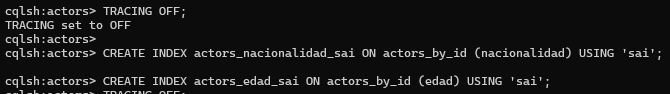
\includegraphics[width=0.75\textwidth]{img/P2_crear_sai.png}
	\caption{Creación de los índices SAI.}
	\label{fig:crearsai}
\end{figure}

Con los índices creados se consultó por nacionalidad, por edad y por ambos atributos.

\begin{lstlisting}
SELECT nombre, nacionalidad, edad FROM actors_by_id WHERE nacionalidad = 'Chile' LIMIT 10;
SELECT nombre, nacionalidad, edad FROM actors_by_id WHERE edad > 60 LIMIT 10;
SELECT nombre, nacionalidad, edad FROM actors_by_id
WHERE nacionalidad = 'Chile' AND edad > 40 LIMIT 10;
\end{lstlisting}

\begin{figure}[H]
	\centering
	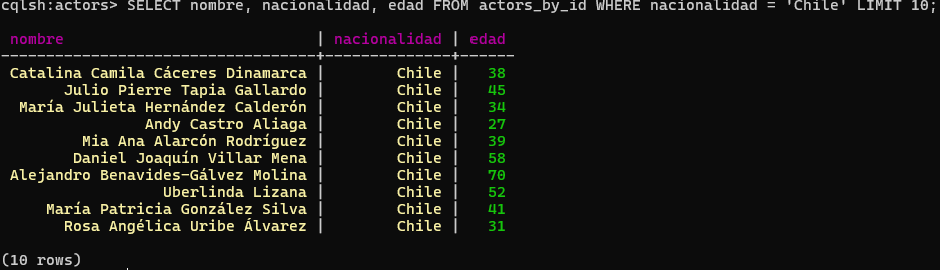
\includegraphics[width=0.75\textwidth]{img/P2_sai_nacionalidad.png}
	\caption{Consulta por nacionalidad usando SAI.}
	\label{fig:sainac}
\end{figure}

\begin{figure}[H]
	\centering
	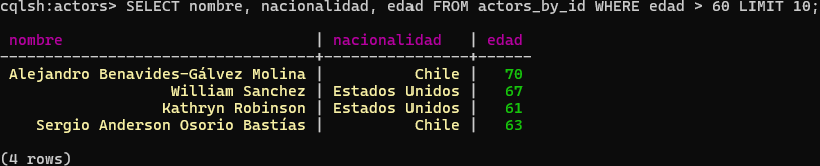
\includegraphics[width=0.65\textwidth]{img/P2_sai_edad.png}
	\caption{Consulta por rango de edad usando SAI.}
	\label{fig:saiedad}
\end{figure}

\begin{figure}[H]
	\centering
	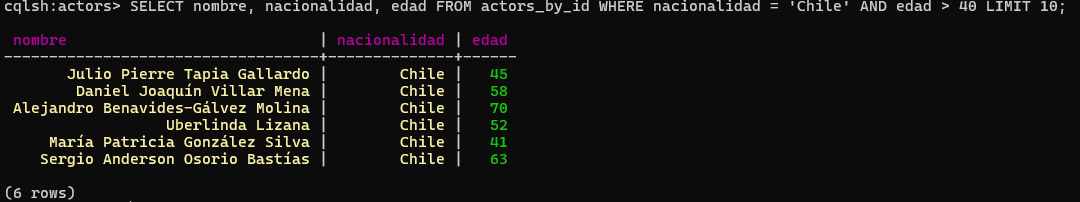
\includegraphics[width=0.85\textwidth]{img/P2_sai_ambas.png}
	\caption{Consulta combinando nacionalidad y edad.}
	\label{fig:saiambas}
\end{figure}

La consulta combinada es la misma que en la sección anterior fue rechazada, y ahora se ejecuta
sin \texttt{ALLOW FILTERING} con los mismos 6 resultados. La consulta por edad muestra que SAI
también permite rangos (\texttt{>} y \texttt{<}) sobre columnas numéricas.

Después se creó un índice sobre los valores de la colección de idiomas y se buscó con
\texttt{CONTAINS}.

\begin{lstlisting}
CREATE INDEX actors_idiomas_sai ON actors_by_id (VALUES(idiomas)) USING 'sai';

SELECT nombre, nacionalidad, idiomas
FROM actors_by_id
WHERE idiomas CONTAINS 'Ingles'
LIMIT 10;
\end{lstlisting}

\begin{figure}[H]
	\centering
	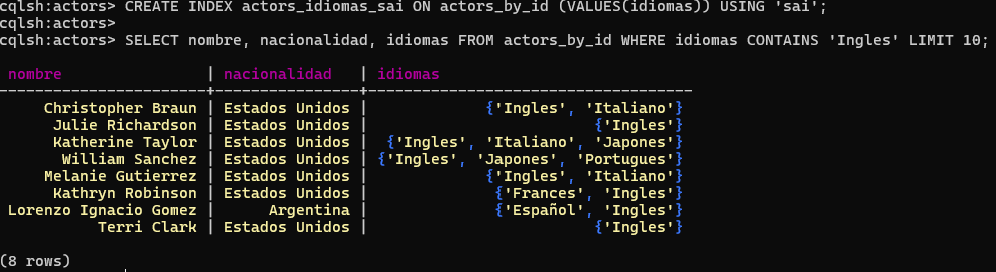
\includegraphics[width=0.8\textwidth]{img/P2_sai_idiomas.png}
	\caption{Búsqueda de actores que hablan inglés con un índice sobre la colección.}
	\label{fig:saiidiomas}
\end{figure}

Para comparar con la búsqueda por clave de partición se repitió la consulta por nacionalidad
con \texttt{TRACING ON}.

\begin{figure}[H]
	\centering
	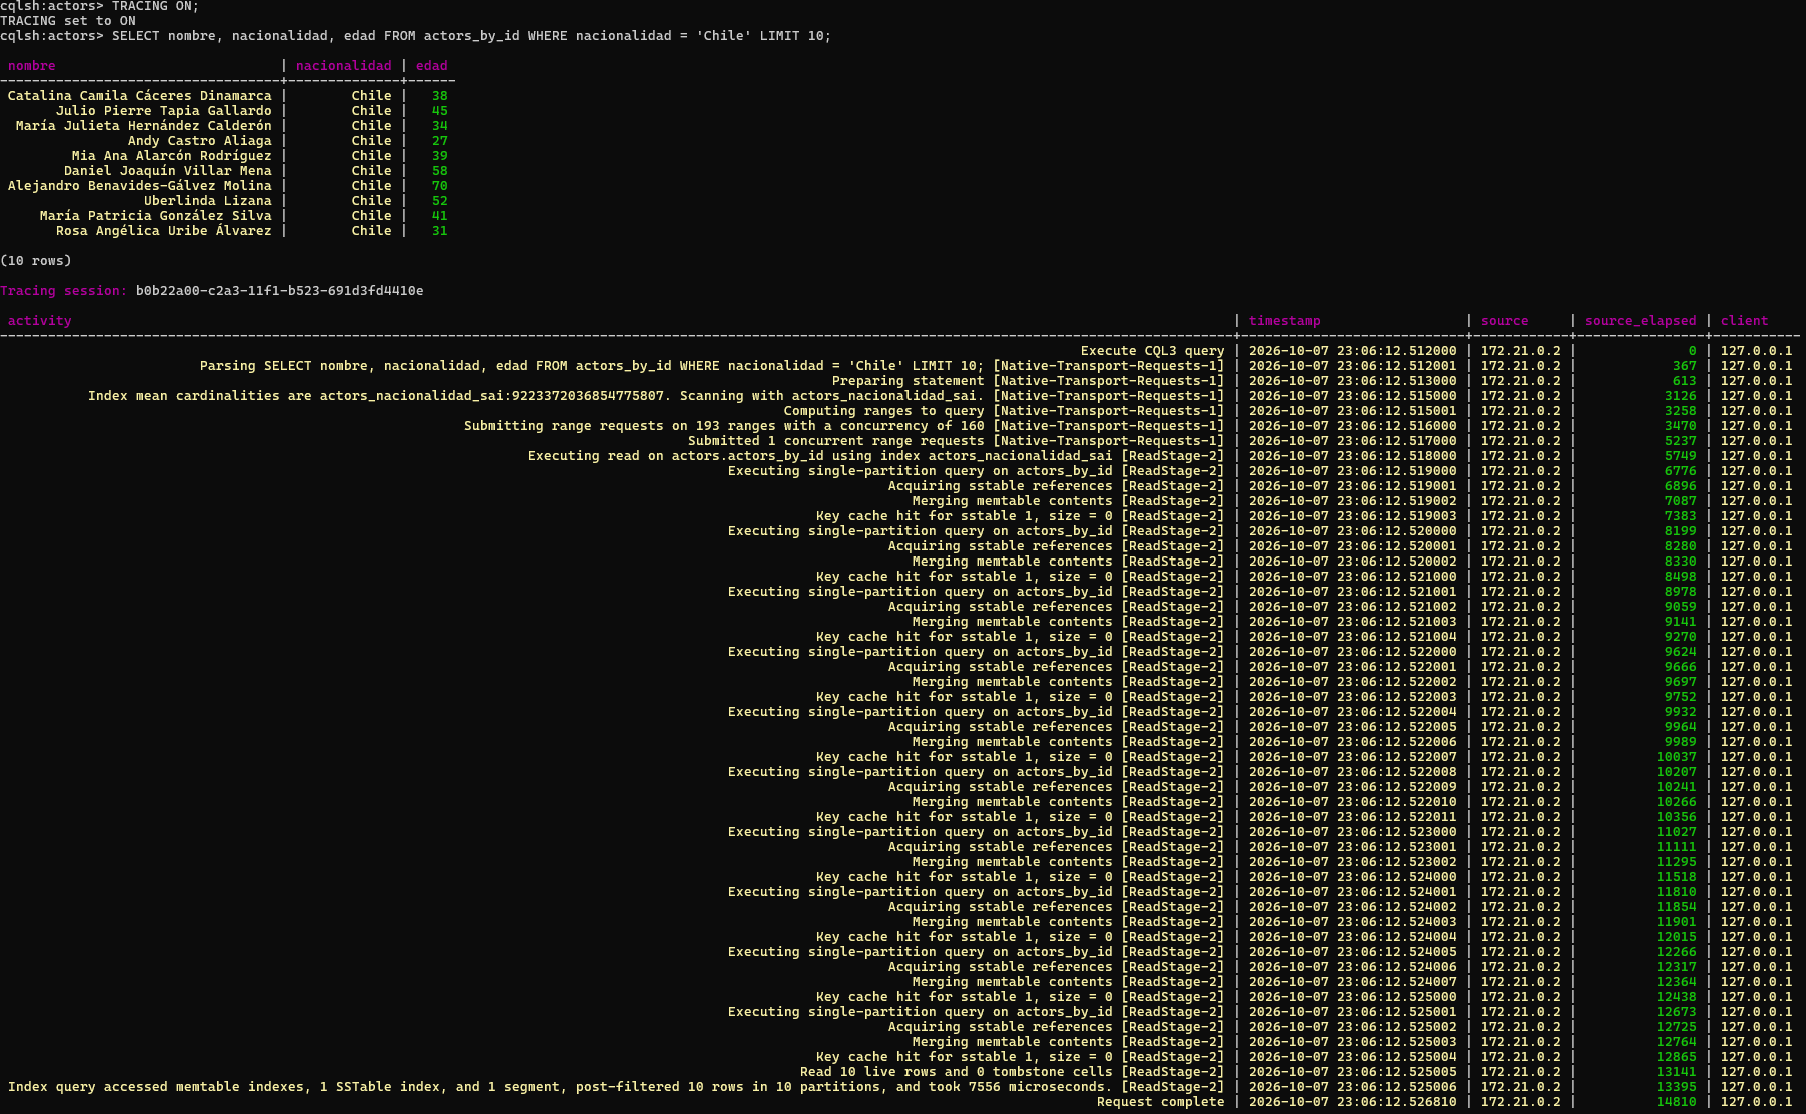
\includegraphics[width=\textwidth]{img/P2_sai_tracing.png}
	\caption{Tracing de la consulta por nacionalidad usando el índice SAI.}
	\label{fig:saitracing}
\end{figure}

El tracing muestra \textit{Scanning with actors\_nacionalidad\_sai}, así que el coordinador
eligió el índice. Igual que con \texttt{ALLOW FILTERING}, aparece
\textit{Submitting range requests on 193 ranges}. Esto pasa porque los índices SAI son
locales: cada nodo indexa solo los datos que guarda, y sin clave de partición hay que
preguntarle al índice de todos los rangos. La diferencia está en lo que se lee después. El
índice indica qué filas cumplen la condición y Cassandra ejecuta una
\textit{single-partition query} por cada una, diez en total, y termina con
\textit{post-filtered 10 rows in 10 partitions}. No leyó filas que no sirvieran. La consulta
tardó 14,8 ms. En este tracing aparece también \textit{Key cache hit for sstable 1}, porque al
crear los índices Cassandra escribió a disco los datos que tenía en memoria.

\textbf{Comparación con la búsqueda por clave de partición.} Una consulta por clave va directo
a una partición en las réplicas que corresponden. Una consulta por SAI tiene que consultar el
índice en todo el anillo y luego hacer una lectura por cada partición encontrada. SAI evita el
recorrido completo de \texttt{ALLOW FILTERING}, pero sigue siendo más cara que una consulta por
clave, y la diferencia crece con la cantidad de nodos y de resultados.

\textbf{Por qué no indexar todo.} Cada índice SAI ocupa espacio en disco junto a cada sstable
y se actualiza en cada escritura de la tabla, por lo que más índices significan escrituras más
lentas y más trabajo durante las compactaciones. Los índices sobre columnas con pocos valores
distintos, como nacionalidad, devuelven muchísimas filas cuando la tabla es grande y terminan
consultando casi todas las particiones. Los índices sirven para consultas ocasionales o para
filtrar dentro de una partición ya conocida, pero no reemplazan una buena clave de partición
para las consultas frecuentes.

\subsection{Desnormalización frente a índices}

Para la misma consulta (actores chilenos) se compararon la tabla diseñada para ella
(Figura~\ref{fig:tracing2}) y la tabla principal con el índice SAI
(Figura~\ref{fig:saitracing}). Se agrega el caso con \texttt{ALLOW FILTERING} como referencia.

\begin{table}[H]
	\centering
	\small
	\begin{tabularx}{\textwidth}{X X X r}
		\toprule
		\textbf{Forma de consulta} & \textbf{Qué consulta} & \textbf{Qué lee} & \textbf{Tiempo} \\
		\midrule
		\texttt{actors\_by\_nationality} & una partición (Chile) & 10 filas contiguas, ya ordenadas por edad & 12,5 ms \\
		\addlinespace
		\texttt{actors\_by\_id} con SAI & los 193 rangos del anillo & 10 particiones distintas, sin orden & 14,8 ms \\
		\addlinespace
		\texttt{actors\_by\_id} con \texttt{ALLOW FILTERING} & los 193 rangos del anillo & las 24 filas de la tabla & 41,6 ms \\
		\bottomrule
	\end{tabularx}
	\caption{Comparación de las formas de consultar por nacionalidad.}
	\label{tab:desnorm}
\end{table}

Con 24 actores los tiempos se parecen, así que la comparación importante es la cantidad de
trabajo.

\textbf{Uso de la clave de partición.} En la tabla desnormalizada la nacionalidad es la clave
de partición, así que la consulta va directo a una partición y además sale ordenada por edad
gracias al clustering. Con SAI la nacionalidad es una columna común, el coordinador no sabe
dónde están los datos y tiene que consultar todos los rangos. El resultado tampoco sale
ordenado por edad, y no se le puede pedir \texttt{ORDER BY edad} porque la edad no es
clustering en esa tabla. Y en cuanto a la \textbf{Duplicación de información.} 
La tabla desnormalizada repite nombre, fecha de
nacimiento, patrimonio e idiomas de cada actor. SAI no duplica las filas, solo guarda la
estructura del índice.

 Con la tabla desnormalizada cada cambio en un dato duplicado se
tiene que escribir en las dos tablas, y es la aplicación la que debe mantenerlas coherentes,
porque Cassandra no lo hace, por lo que hay un \textbf{costo de mantención.}. 
Un cambio de edad es más caro todavía: como la edad es parte de
la clave de \texttt{actors\_by\_nationality}, no se puede actualizar, hay que borrar la fila y
volver a insertarla. Con SAI la mantención la hace Cassandra, que actualiza el índice en cada
escritura, pero eso agrega costo a todas las escrituras de la tabla.

\textbf{Índices adicionales.} Si se quisiera consultar por otras columnas habría que elegir
entre crear más tablas desnormalizadas (más espacio y más escrituras por cada cambio) o más
índices (consultas que recorren el anillo y escrituras más lentas). En general, para una
consulta frecuente conviene la tabla diseñada para ella, y los índices quedan para consultas
ocasionales.

\subsection{Escalabilidad}

Si la base tuviera 10 mil millones de registros el comportamiento de cada tipo de consulta
cambiaría de la siguiente forma.

En cuanto a las \textbf{Consultas por clave de partición y clustering.} Siguen yendo directo a las réplicas de
una partición, así que su costo depende del tamaño de esa partición y no del total de la
tabla. La búsqueda por \texttt{actor\_id} se mantendría prácticamente igual. El problema
aparece en \texttt{actors\_by\_nationality}: con 10 mil millones de actores la partición de un
país podría tener cientos de millones de filas, todas en los mismos tres nodos. Eso genera una
partición demasiado grande y un punto caliente en el clúster. Se resolvería con una clave de
partición compuesta, por ejemplo \texttt{((nacionalidad, rango\_edad), edad, actor\_id)}, que
reparte un mismo país entre varias particiones más pequeñas.

Si se quisieran hacer \textbf{consultas con ALLOW FILTERING.} Tendrían que leer los 10 mil millones de filas para
quedarse con las que cumplen la condición. El tiempo crecería con el total de datos, la
consulta superaría los timeouts y afectaría a todos los nodos del clúster mientras se ejecuta.
En la práctica no serían utilizables.

La \textbf{consultas mediante SAI} evitan leer filas que no cumplen el filtro, pero siguen
consultando el índice en todos los nodos. Funcionan bien cuando el filtro es selectivo y
devuelve pocas filas. Con un filtro poco selectivo, como una nacionalidad con millones de
actores, el coordinador tendría que reunir resultados de todo el clúster y hacer una lectura
por cada partición encontrada. Rinden mucho mejor si se combinan con la clave de partición,
porque así el índice solo se consulta dentro de esa partición.

\textbf{Cantidad de particiones o nodos consultados.} Una consulta por clave de partición
consulta solo las réplicas de esa partición, que con RF = 3 son tres nodos como máximo, y con
consistencia ONE basta uno, sin importar cuántos nodos tenga el clúster. \texttt{ALLOW
FILTERING} y SAI sin clave de partición consultan todos los rangos del anillo, así que si el
clúster crece a cientos de nodos para guardar los datos, estas consultas tienen que hablar con
todos ellos.

Y en \textbf{almacenamiento.} Con RF = 3 cada fila se guarda tres veces. La desnormalización
multiplica eso: los datos de cada actor están en \texttt{actors\_by\_id} y en
\texttt{actors\_by\_nationality}, así que con 10 mil millones de actores habría unas seis
copias de esa información en el clúster. Cada índice SAI agrega su propio espacio en cada
réplica. En Cassandra se acepta pagar más disco para que las lecturas sean simples, pero eso
hay que tenerlo presente al dimensionar el clúster.

\textbf{Por qué conocer las consultas antes.} En Cassandra la clave primaria decide dónde se
guardan los datos y en qué orden, y no se puede cambiar después de crear la tabla. Si aparece
una consulta que no coincide con ninguna clave, las únicas salidas son \texttt{ALLOW
FILTERING}, que no escala, un índice, que tiene costo en todo el clúster, o crear una tabla
nueva y volver a cargar todos los datos. Por eso el diseño parte de la lista de consultas de
la aplicación y no del modelo de entidades, al revés de lo que se hace en una base relacional.

\section{Parte 3: Comparación, alta disponibilidad y actualización}

\section{Parte 4: Cierre}

\section{Referencias y material complementario}

\begin{itemize}
	\item Apache Cassandra Documentation. \emph{Data Modeling}.
	\item Apache Cassandra Documentation. \emph{CQL: Data Manipulation (SELECT, ALLOW FILTERING)}.
	\item Apache Cassandra Documentation. \emph{Storage-Attached Indexing (SAI)}.
	\item Apache Cassandra Documentation. \emph{Tracing}.
	\item Enlace al repositorio público: \url{https://github.com/Sxbayb/Tareas-BDDA}.
	\item Material de clase. 2.3 Bases de Datos de Columnas Anchas.
\end{itemize}

\end{document}
